\chapter{Experiments}
\label{chapter:evaluation}


\section{Overview}
In this chapter, we start with exploring how we evaluate the experiments and what metrics we use to measure them in Section \ref{section:eval}. Next, in Section \ref{section:trit} we discuss the experimental setup and the system used for the experiments. To better understand the impact of data in ASR experiments, we run multiple training configurations using different amounts of data in Section \ref{section:res_scale}. Then, in Section \ref{section:res_dist} we analyse the impact of distributed training and evaluate the impact of using multi \acrshort{gpu}, multiprocess techniques on training time and \acrshort{wer}. In the end, we try to match hyperparameters of distributed training exactly with normal training to check the direct time comparisons of convergence time. 


\section{Experimental Setup}
\label{section:trit}
For all of our experiments, we use Aalto University's Triton\footnote{Triton cluster, Aalto scientific computing \href{https://scicomp.aalto.fi/triton/}{https://scicomp.aalto.fi/triton/}}, a high-performance computing cluster. Triton has an Nvidia DGX-1\footnote{Nvidia DGX, Wikipedia \href{https://en.wikipedia.org/wiki/Nvidia_DGX}{https://en.wikipedia.org/wiki/Nvidia\_DGX}} machine which contain 8 Tesla V100 \acrshort{gpu}s and are optimized for deep learning applications. Each GPU has a 16 GB memory with CUDA compute 7.0 capability. These \acrshort{gpu}s are used for all the deep learning training jobs, including the multi-\acrshort{gpu} ones. This research work also required large amounts of storage that can be accessed from multi processes and from multiple nodes at the same time, we use the Lustre\footnote{Lustre \href{https://www.lustre.org/}{https://www.lustre.org/}} filesystem which is a scalable filesystem which provides large storage capacity and high sequential throughput for cluster-based applications. The lustre storage is connected via an Infiniband\footnote{InfiniBand, Wikipedia. \href{https://en.wikipedia.org/wiki/InfiniBand}{https://en.wikipedia.org/wiki/InfiniBand}} connection, which features high throughput and low latency.

\section{Evaluation Criteria}
\label{section:eval}
We monitor the training jobs using TensorBoard. The main metrics that are tracked are training loss value, validation loss value and validation \acrshort{wer}. The input transcript follows the typical conventions for capitalization and punctuation, as discussed in Section \ref{section:bizspeech}. In the initial stages of experiments, we did not take steps to remove punctuation marks and capitalization from the input text, and this led to the acoustic model being trained end to end along with the capitalization and punctuation marks in them. Hence, for the later experiments, we stuck with this setup because we noticed that the model was able to predict the capitalization and punctuation marks in many cases. During post-processing, we apply text normalization and report word error rates, based on the test split of the dataset, with and without punctuations or capitalization. Therefore, for all experiments we have a \acrshort{wer} with punctuations considered and without punctuations in them. We also report the \acrlong{cer} with punctuations for the test set. The train, validation, and test data splits details are shown in the Table \ref{table:splits}.

\begin{table}[ht]
\centering
\begin{tabular}{ c | c  c }
\hline
  & Utterances & Hours \\
 \hline
 \verb|Train| & 8809282 & 20000 \\ 
 %\hline
 \verb|Validation| & 186165 & 413 \\ 
 %\hline
 \verb|Test| & 185623 & 412 \\ 
 \hline
\end{tabular}
\caption{\label{table:splits}Dataset Train Validation Test Statistics }
\end{table}

\section{Experiments overview}
\label{section:exp_desc}
We use \inlinecode{SentencePiece} Tokenizer with vocabulary size of 5k with \emph{bpe} as the token type. The detokenized output from the acoustic model consists of upper case characters, lower case characters, digits, punctuation marks, percent sign, currency notations, space character, a token for silence, hence covering all the characters present in the dataset transcriptions. The model used is an attention-based encoder decoder model. For the encoder, we use a \acrshort{crdnn} model. The convolution part of the \acrshort{crdnn} model has 2  blocks. Each block has 2 convolution layers with \inlinecode{LayerNorm} applied and \inlinecode{LeakyReLU} activation function. These two convolution layers are then followed by \inlinecode{MaxPool} and \inlinecode{Dropout} layers. The two major blocks are chained together, and then the output is passed to a bidirectional-\acrshort{lstm} cell with 512 neurons. The output of the recurrent part of the neural network is then passed to the \acrshort{mlp} portion of the network. This has two blocks of Linear Layer with \inlinecode{BatchNorm} and \inlinecode{LeakyReLU} activation function with \inlinecode{Dropout}. We then use the output of the encoder with an embedding layer, which is a \inlinecode{Linear} layer. The output of the embedding layer is then fed to the decoder part of the network. The decoder is a location aware attentional \acrshort{rnn} with a \acrshort{gru} cell with the attention dimension set to 512. The complete model architecture is given in the Appendix \ref{chapter:model-architecture}. We use Adam optimizer with learning rate set to 0.0001 without any scheduler. We apply \acrshort{ctc} loss for the initial 15 epochs and then disabled it for further training. and complete hyperparameter configuration in \ref{chapter:hyparam}. The best validation word error rate was used as the final model. The target batch size used was 180 seconds, with a maximum batch size of 240 seconds. The batch size is represented in seconds because of the dynamic batching method explained in Section \ref{section:dynbatch}. No language models were used to evaluate the final metrics.  

\section{Dataset size-based experiments}
\label{section:res_scale}
We performed experiments to compare the models between the different scales of data used for training jobs. We run training jobs using 80, 200, 2000, 8000 and 20000 hours. For all the data scales, we spawn two processes for data loading and preprocessing. The different dataset splits that were used are shown in Table \ref{table:datascales}.

\begin{table}[ht]
\centering
\begin{tabular}{c c c c c}
\hline
  Hours & Training Utterances & WER & WER-P & CER-P\\
 \hline
  80 & 38246 & 46.73\% & 50.38\% & 29.63\%\\ 
  200 & 94840 & 43.84\% & 47.84\% & 29.08\%\\
  2000 & 964824 & 33.76\% & 38.52\% & 27.8\%\\
  8000 & 3480514 & 20.74\% & 24.31\% & 12.04\%\\
  20000 & 8809282 & 14.01\% & 17.12\% & 7.67\%\\
 \hline
\end{tabular}
\caption{\label{table:datascales}Dataset Split for training at different scales. WER is word error rate without punctuations, WER-P is the word error rate considering the punctuations and capitalizations, CER-P is the character error rate with the punctuations and capitalizations. }
\end{table}

Note that for evaluation, the same test and validation sets are used across all the scales to make it convenient to compare the results. Because the test and validation splits are made with the largest dataset in mind, they are larger than the training sets for 80 and 200 hour datasets. Predictably, the word error rates drop with the increase in the scale of training data, and the similar trend is seen with the character error rates. The difference between the word error rates with and without punctuation is at an almost constant 3.5\% points. The CER-P is also an important metric for our dataset because of the presence of punctuation and capitalization in the transcript.

\section{Distributed Training}
\label{section:res_dist}
All the experiments discussed above are run using a single GPU and a single process. This section now delves into the distributed training experiments. 

\subsection{Synchronous training}
\acrfull{ddp} approach is used for synchronous training. In these experiments, we spawn 4 processes, each with access to a discrete GPU. The same model is copied to all the \acrshort{gpu}s. Each process computes the forward pass and the loss and gradients to backpropogate, and for each GPU, we also spawn two processes for data loading and preprocessing on the fly. For using multiple \acrshort{gpu}s, the batch size becomes a vital hyperparameter. If we retain the same batch size as that was used for the single \acrshort{gpu}, the overall effective batch size is the number of GPUs used times the single batch size. The word error rates for these experiments are reported in Table \ref{table:wer_ddp}. For the \acrshort{ddp} experiments, we use 4 GPUs with the effective batch size is multiplied by 4 times. 

\begin{table}[ht]
\centering
\begin{tabular}{c | c c c | c c c }
\hline
\textbf{Training Dataset} & \multicolumn{3}{c|}{\textbf{8000}} & \multicolumn{3}{c}{\textbf{20000}}\\\cline{2-7}
   \textbf{Size (in hrs)} & WER & WER-P & CER-P & WER & WER-P & CER-P\\
 \hline
  Single GPU & 20.74\% & 24.31\% & 12.04\% & 14.01\% & 17.12\% & 7.67\%\\
  4-GPU DDP & 17.38\% & 20.65\% & 10.16\% & 10.87\% & 13.69\% & 5.73\% \\
 \hline
\end{tabular}
\caption{\label{table:wer_ddp} WER, WER-P and CER-P comparison for single GPU and multi GPU runs.}
\end{table}

We compare the distributed data parallel results with the single GPU results. We observe improvement of 15\%-38\% in \acrshort{wer}. This can be attributed to the fact that larger batch sizes work better for the hyperparameter configuration and model architecture setup because everything apart from that is kept constant. Hence, the use of DDP is perfect for these experiments since it enables usage of larger batch sizes. From these experiments, it is apparent that using DDP is beneficial, especially in cases where larger batch sizes lead to better convergence of the models. 


\begin{table}[ht]
\centering
\begin{tabular}{c | c c c | c }
\hline
     & WER & WER-P & CER-P & Training Wall-time (hrs)\\
 \hline
  1-GPU & 20.74\% & 24.31\% & 12.04\% & \textbf{59} \\
  1-GPU \acrshort{sga} & 16.74\% & 19.98\% & 7.60\% & \textbf{80} \\
  4-GPU DDP & 17.38\% & 20.65\% & 7.67\% & \textbf{42} \\
 \hline
\end{tabular}
\caption{\label{table:wer_ddp_grad} WER, WER-P and CER-P comparison for single GPU, single GPU with sequential gradient accumulation and multi GPU runs for the 8000 training hours dataset. The table also shows the wall clock time to convergence with the different setups.}
\end{table}

Hence, to make comparisons on the time to convergence of the models, we try to level the batch sizes for the two setups. One way would be to reduce the batch size by a factor of the number of GPUs used for the DDP setup. However, this means that the efficiency of the training is reduced. Therefore, we choose a different method to achieve consistency between the setups. Since the gradients in the multiple GPU setup are updated 4 batches at a time by computing them in parallel, we apply the backward pass after accumulating the gradients for 4 batches, processed sequentially using a single \acrshort{gpu}. This effectively means that the batch size is increased by a factor of 4. We call this method \acrfull{sga}. In this method, we compute the forward pass, the loss, and the gradients for four batches sequentially and then run the backward pass once after accumulating them across the four batches. This makes the comparison more fair and easier to make. This experiment is conducted for the 8000 training hour dataset to get the results faster. We expect similar results with the larger dataset as well. 

\begin{figure}[ht]
  \begin{center}
    % below the size of the figure has been reduced for example
    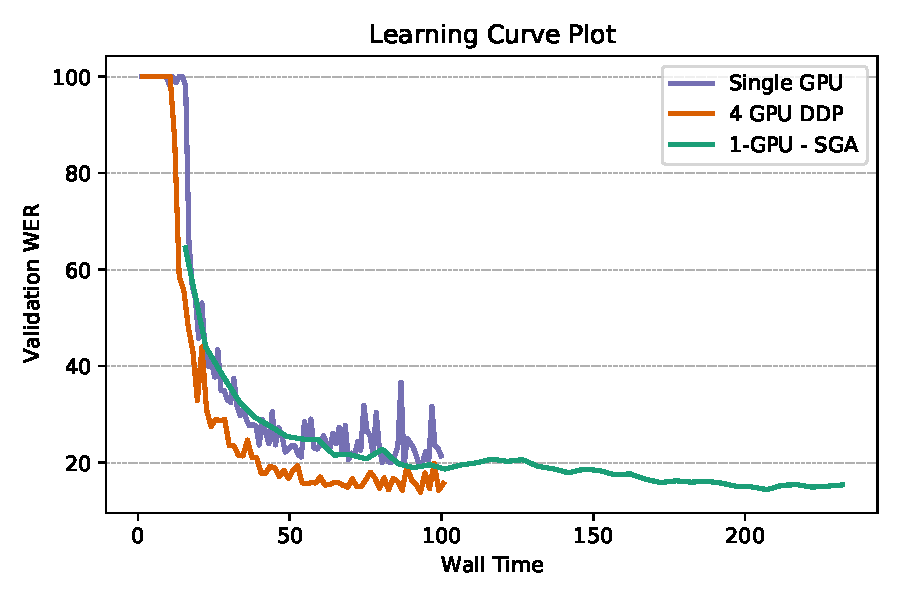
\includegraphics[width=\textwidth]{images/learning_curve_8000.pdf} 
    \caption{Learning curves during training for the different setups, with Validation WER on the y-axis and wall clock time in hours on the x-axis.}
    \label{fig:learningcurve_ddp}
  \end{center}
\end{figure}


The word error rate for the \acrshort{sga} experiment is compared with the other results in the Table \ref{table:wer_ddp_grad}. We see that the word error rates differ by around 0.5\% points between the \acrshort{sga} and the \acrshort{ddp} methods, and this can be attributed to minute variations like initial seeds and other random occurrences. The time to convergence is also reported in the same table. This is measured by having a benchmark \acrshort{wer} of 19.74\%, which is the Azure's WER on random utterances from the dataset, discussed in Section \ref{section:bizspeech}. So, \emph{time to convergence here is defined as the training wall clock time for the model to reach the validation word error rate of 19.74\%}. We see that the single GPU run reached the benchmark \acrshort{wer} at around the 60 hours mark, which is 1.5 times the time to convergence of the 4-GPU DDP, but the single GPU model doesn't converge overall as much as the DDP run. Comparing the 1-GPU \acrshort{sga} and the 4-GPU \acrshort{ddp}, the time to convergence is reduced by half. The single GPU SGA takes 80 hours to reach the benchmark WER. Figure \ref{fig:learningcurve_ddp} shows the learning curve for the three runs, with the validation word error rate on the y-axis and wall clock time in hours on the x-axis. Note that the training was stopped when the training loss was stagnant over at least 5 epochs. Again we see that the DDP plot reaches the benchmark \acrshort{wer} the quickest and converges sharply in the initial hours. 

\subsection{Asynchronous training}
Hogwild \cite{Niu2011HOGWILD:Descent} is used to evaluate the usage of asynchronous training. In this experiment, we store the weights on one single GPU, and we spawned 3 different processes to process the forward pass over different batches of data and calculate the loss and gradients to backpropogate. Then each process continues to update the weights on the GPU. Next, all individual processes again read the updated weights and continues to iterate over the next batches of data. We use 2 processes for each main process for data loading and preprocessing. Overall, the system works without any interlocking mechanism to ensure that the updates to the model weights are actually read by the other processes before being overwritten. Again, the batch size is a crucial hyperparameter because all the 3 processes use the same GPU, the same batch size as single process cannot be used as we will face issues managing the GPU memory. If we reduce the batch size for the single process experiment, the device efficiency reduces. The word error rates for these experiments are reported in Table \ref{table:wer_hog}. For the Hogwild experiments, we use 3 processes, and thus the effective batch size is divided by 3 times. 

\begin{table}[ht]
\centering
\begin{tabular}{c | c c c | c c c }
\hline
\textbf{Training Dataset} & \multicolumn{3}{c|}{\textbf{8000}} & \multicolumn{3}{c}{\textbf{20000}}\\\cline{2-7}
   \textbf{Size (in hrs)} & WER & WER-P & CER-P & WER & WER-P & CER-P\\
 \hline
  Single Process & 20.74\% & 24.31\% & 12.04\% & 17.38\% & 20.65\% & 10.16\%\\
  3-Process Hogwild & 22.4\% & 25.7\% & 12.70\% & 24.09\% & 27.56\% & 13.81\% \\
 \hline
\end{tabular}
\caption{\label{table:wer_hog} WER, WER-P and CER-P comparison for single process and multiprocess Hogwild runs for two data scales}
\end{table}

We compare the Hogwild results with the single GPU results. We observe a deterioration of 8\%-38\% in \acrshort{wer} with using Hogwild. This can be attributed to the fact that smaller batch sizes work does not work well for the hyperparameter configuration and model architecture setup because all the other configurations is kept constant. Hogwild also doesn't improve by adding more data. We see that the accuracy metrics are better for the 8000 hours training set. Similar to the synchronous training experiments, comparing these results which have different effective batch sizes is not reasonable. 

\begin{table}[ht]
\centering
\begin{tabular}{c | c c c | c }
\hline
     & WER & WER-P & CER-P & Training Wall Time (hrs)\\
 \hline
  1-Process & 20.74\% & 24.31\% & 12.04\% & \textbf{35} \\
  1-Process $\frac{1}{3}$ BS & 24.16\% & 27.75\% & 14.91\% & \textbf{54} \\
  3-Process Hogwild & 22.4\% & 25.7\% & 12.70\% & \textbf{46} \\
 \hline
\end{tabular}
\caption{\label{table:wer_hog_seq} WER, WER-P and CER-P comparison for single GPU, single GPU with sequential gradient accumulation and multi GPU runs for the 8000 training hours dataset. The table also shows the wall clock time to convergence with the different setups.}
\end{table}

Hence, to make the comparisons on the time to convergence of the models, we use sequential updates to simulate multiple process settings on a single process system. We reduce the batch size of the single process experiment to one third the size of the regular batch size, and this equates it to the Hogwild experiment closely. This makes the comparison more fair and easier to make. This experiment is conducted for the 8000 training hour dataset to get the results faster.  We expect similar results with the larger dataset as well. Since Hogwild never reaches \acrshort{wer} of 19.74\%, we use a word error rate of 30\% as the benchmark to compare the time of convergence. The word error rate for the single process with reduced batch size is compared with the other results in Table \ref{table:wer_hog_seq} along with  wall time to convergence (at 30\% WER) in hours. We see that Hogwild does slightly better in word error rates and character error rates than the sequential update with reduced batch size. This can be due to the different processes updating the gradients in different batches in parallel, thus exploring more of the gradient space and the algorithm can find a better optima. Comparing the time to convergence, we see that the single process run converges quickest, but along the experiments which uses the same effective batch size, Hogwild converges around 8 hrs quicker than the sequential update simulation of Hogwild. 

\begin{figure}[ht]
  \begin{center}
    % below the size of the figure has been reduced for example
    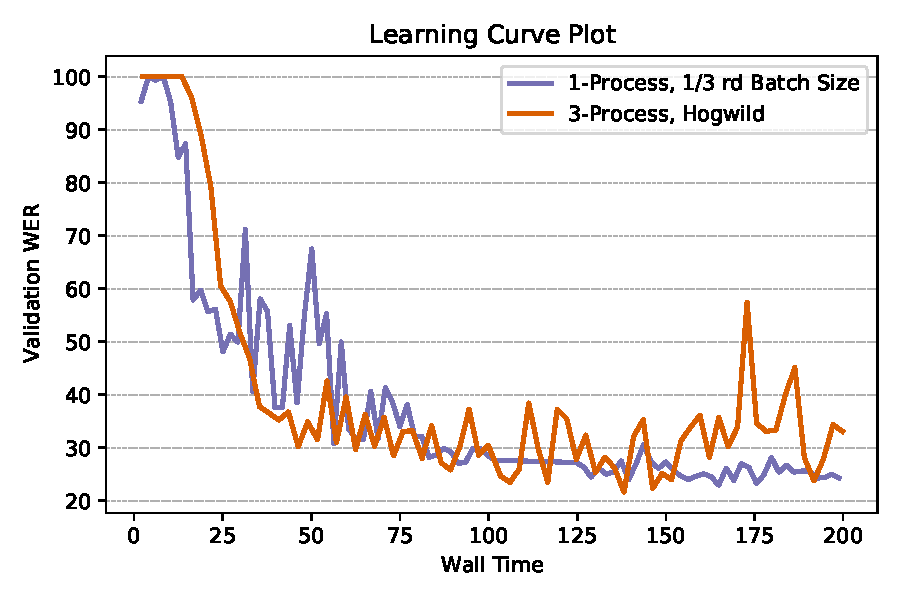
\includegraphics[width=\textwidth]{images/learning_curve_8000_hogwild.pdf} 
    \caption{Learning curves during training for the different setups, with Validation WER on the y-axis and wall clock time in hours on the x-axis.}
    \label{fig:learningcurve_async}
  \end{center}
\end{figure}

Figure \ref{fig:learningcurve_async} shows the learning curve for the two runs, with the validation word error rate on the y-axis and wall clock time in hours on the x-axis. Note that the training was stopped when the training loss was stagnant over at least 5 epochs. The learning curves are quite erratic, and we observe a lot of variation in validation word error rates even when the training loss vales are constant. 
